\documentclass[12pt,a4paper]{article}
\raggedbottom

\usepackage{ugmath}
\usepackage{float}
\usepackage{placeins}
\usepackage[labelfont=bf,labelsep=space]{caption}
\usepackage{pdfpages}
\usepackage{tikz-cd}
\usepackage{amsthm}
\renewcommand{\Tr}{\operatorname{Tr}}
\newcommand{\llaves}[1]{\{#1\}}
\newcommand{\parentesis}[1]{\left(#1\right)}
\newcommand{\corchetes}[1]{\left[#1\right]}
\newcommand{\llavesgrande}[1]{\big\{#1\big\}}
\newcommand{\llavesgrandes}[1]{\left\{#1\right\}}


\begin{document}
        
    \thispagestyle{empty}
    
\includepdf[pages=1]{main.pdf}

    \begin{problema}
        Prueba el inciso (b) de la proposición 6.
    \end{problema}

    \begin{proof}
        Sea $x\in\R$ con $x\neq0$ y supongamos que $y\in\R$ cumple
        \begin{equation*}
            xy=1.
        \end{equation*}
        Multiplicando ambos lados por $x^{-1}$ obtenemos
        \begin{equation*}
            x^{-1}(xy)=x^{-1}\cdot1.
        \end{equation*}
        Por la asociatividad del producto y la definición de $x^{-1}$, el lado izquierdo es $(x^{-1}x)y=1\cdot y=y$, y por la propiedad del neutro multiplicativo el lado derecho es $x^{-1}$. Así,
        \begin{equation*}
            y=x^{-1}.
        \end{equation*}
        Por lo tanto, el único número que cumple $x\cdot y=1$ es $x^{-1}$.
    \end{proof}

    \begin{problema}
        Sean $x$ y $y$ números reales distintos de cero. Prueba, usando la unicidad del inverso multiplicativo, que
        \begin{equation*}
            (xy)^{-1}=x^{-1}y^{-1}.
        \end{equation*}
    \end{problema}

    \begin{proof}
        Como $x\neq0$ y $y\neq0$, se tiene $xy\neq0$ (pues si $xy=0$ entonces $x=0$ o $y=0$), de modo que $(xy)^{-1}$ existe y, por definición,
        \begin{equation*}
            (xy)(xy)^{-1}=1.
        \end{equation*}
        Multiplicando por $x^{-1}$ y usando la asociatividad y la conmutatividad,
        \begin{equation*}
            (x^{-1}x)\,y\,(xy)^{-1}=x^{-1}
            \quad\Longrightarrow\quad
            y\,(xy)^{-1}=x^{-1}.
        \end{equation*}
        Multiplicando ahora por $y^{-1}$,
        \begin{equation*}
            (y^{-1}y)\,(xy)^{-1}=x^{-1}y^{-1}
            \quad\Longrightarrow\quad
            (xy)^{-1}=x^{-1}y^{-1}.
        \end{equation*}
    \end{proof}

    \begin{problema}
        \textbf{(Aritmética de las fracciones)} Sean $x$, $y$, $z$ y $w$ números reales tales que las expresiones algebraicas de los incisos siguientes
        están definidas. Prueba lo siguiente:
        \begin{enumerate}
            \item[(a)] $\dfrac{x}{y}+\dfrac{z}{w}=\dfrac{wx+yz}{yw}.$
            \item[(b)] $\dfrac{x}{y}-\dfrac{z}{w}=\dfrac{wx-yz}{yw}.$
            \item[(c)] $\dfrac{x}{y}\cdot\dfrac{z}{w}=\dfrac{xz}{yw}.$
            \item[(d)] $\dfrac{x}{y}\mathbin{\divisionsymbol}\dfrac{z}{w}=\dfrac{xw}{yz}.$
        \end{enumerate}
        \textbf{Sugerencia:} Recuerda cómo se definió la resta y la división de números reales.
    \end{problema}

    \begin{proof}
        En todos los incisos usamos que $\dfrac{a}{b}=ab^{-1}$ y que, por el problema 2, $(yw)^{-1}=y^{-1}w^{-1}$.
        \begin{enumerate}
            \item[(a)] Partimos del lado derecho:
            \begin{align*}
                \frac{wx+yz}{yw}&=(wx+yz)(yw)^{-1}\\
                &=wx(yw)^{-1}+yz(yw)^{-1}\\
                &=wx\,y^{-1}w^{-1}+yz\,y^{-1}w^{-1}\\
                &=(w\,w^{-1})(x\,y^{-1})+(y\,y^{-1})(z\,w^{-1})\\
                &=1\cdot(x\,y^{-1})+1\cdot(z\,w^{-1})\\
                &=xy^{-1}+zw^{-1}\\
                &=\frac{x}{y}+\frac{z}{w}.
            \end{align*}
            \item[(b)] Por definición de la resta, $wx-yz=wx+(-(yz))$, y por las leyes de los signos $(-(yz))(yw)^{-1}=-\left(yz(yw)^{-1}\right)$. Entonces
            \begin{align*}
                \frac{wx-yz}{yw}&=(wx-yz)(yw)^{-1}\\
                &=wx(yw)^{-1}-yz(yw)^{-1}\\
                &=(w\,w^{-1})(x\,y^{-1})-(y\,y^{-1})(z\,w^{-1})\\
                &=xy^{-1}-zw^{-1}\\
                &=\frac{x}{y}-\frac{z}{w},
            \end{align*}
            donde el tercer paso se justifica igual que en el inciso (a).
            \item[(c)] Partimos del lado izquierdo:
            \begin{align*}
                \frac{x}{y}\cdot\frac{z}{w}&=(xy^{-1})(zw^{-1})\\
                &=(xz)(y^{-1}w^{-1})\\
                &=(xz)(yw)^{-1}\\
                &=\frac{xz}{yw}.
            \end{align*}
            \item[(d)] Por definición de la división, y como $z\neq0$ y $w\neq0$,
            \begin{align*}
                \frac{x}{y}\mathbin{\divisionsymbol}\frac{z}{w}&=(xy^{-1})(zw^{-1})^{-1}\\
                &=(xy^{-1})\left(z^{-1}(w^{-1})^{-1}\right)\\
                &=(xy^{-1})(z^{-1}w)\\
                &=(xw)(y^{-1}z^{-1})\\
                &=(xw)(yz)^{-1}\\
                &=\frac{xw}{yz},
            \end{align*}
            donde usamos $(zw^{-1})^{-1}=z^{-1}(w^{-1})^{-1}$ (problema 2) y $(w^{-1})^{-1}=w$.
        \end{enumerate}
    \end{proof}

    \begin{problema}
        Prueba que si $x,y\geq0$ y $x+y=0$, entonces $x=0$ y $y=0$.
    \end{problema}

    \begin{proof}
        Sean $x,y\geq0$ con $x+y=0$ y supongamos, por contradicción, que $x\neq0$ o $y\neq0$. Como ambos son no negativos, al menos uno de ellos es positivo.
        Si $x\gt0$, como $y\geq0$ se tiene
        \begin{equation*}
            x+y\geq x+0=x\gt0,
        \end{equation*}
        lo que contradice $x+y=0$. Si $y\gt0$, como $x\geq0$ se tiene
        \begin{equation*}
            x+y\geq0+y=y\gt0,
        \end{equation*}
        lo que también contradice $x+y=0$. Por lo tanto, la suposición es falsa y
        \begin{equation*}
            x=0\quad\text{y}\quad y=0.
        \end{equation*}
    \end{proof}

    \begin{problema}
        Determina si existe el supremo de los conjuntos siguientes (argumenta tu respuesta). En caso de que exista, calcúlalo (argumenta tu respuesta).
        Para resolver este ejercicio puedes usar la proposición 17 en los incisos (c) y (d); la proposición 18 en el inciso (e) y la proposición 21 en los incisos (f) y (g).
        \begin{multicols}{2}
            \begin{enumerate}
                \item[(a)] $(-3,5).$
                \item[(b)] $(-3,5].$
                \item[(c)] $\N.$
                \item[(d)] $(0,\infty).$
                \item[(e)] $\llavesgrandes{1-\dfrac{1}{n}:n\in\N}.$
                \item[(f)] $\Q\cap\left(0,\sqrt{2}\right).$
                \item[(g)] $\mathbb{I}\cap(0,1).$
            \end{enumerate}
        \end{multicols}
    \end{problema}

    \begin{solucion}
        \begin{enumerate}
            \item[(a)] Sea $S=(-3,5)$. Para todo $x\in S$ se cumple $x\lt5$, luego $5$ es cota superior de $S$. Sea $u\lt5$ y supongamos que $u$ es cota superior de $S$.
            Si $u\leq-3$, entonces $0\in S$ y $0\gt-3\geq u$, lo cual contradice que $u$ sea cota superior. Si $-3\lt u\lt5$, consideremos
            \begin{equation*}
                x=\frac{u+5}{2},
            \end{equation*}
            que satisface $u\lt x\lt5$; en particular $x\gt-3$, así que $x\in S$ y $x\gt u$, lo cual también contradice que $u$ sea cota superior.
            Por tanto, ninguna $u\lt5$ es cota superior y
            \begin{equation*}
                \sup(-3,5)=5.
            \end{equation*}
            Notemos que $5\notin S$, por lo que $S$ no tiene máximo.
            \item[(b)] Sea $T=(-3,5]$. Para todo $x\in T$ se cumple $x\leq5$, así que $5$ es cota superior de $T$. Además $5\in T$, es decir, $5$ es una cota superior que pertenece a $T$; toda cota superior $u$ de $T$ satisface $5\leq u$, de modo que $5$ es la menor de las cotas superiores. Por tanto,
            \begin{equation*}
                \sup T=5,
            \end{equation*}
            y además $5$ es el máximo de $T$.
            \item[(c)] Supongamos que existe $M\in\R$ cota superior de $\N$. Por la propiedad arquimediana existe $n\in\N$ tal que $n\gt M$, lo cual contradice que $M$ sea cota superior. Así, $\N$ no está acotado superiormente y
            \begin{equation*}
                \sup\N\ \text{no existe en }\R.
            \end{equation*}
            \item[(d)] Sea $M\in\R$ arbitrario y tomemos $x=|M|+1$. Entonces $x\gt0$, es decir, $x\in(0,\infty)$, y además $x\gt|M|\geq M$. Luego ningún $M\in\R$ es cota superior de $(0,\infty)$, y
            \begin{equation*}
                \sup(0,\infty)\ \text{no existe en }\R.
            \end{equation*}
            \item[(e)] Sea $S=\llavesgrandes{1-\dfrac{1}{n}:n\in\N}$. Para cada $n\in\N$ se tiene
            \begin{equation*}
                1-\frac{1}{n}\lt1,
            \end{equation*}
            luego $1$ es cota superior de $S$. Sea $u\lt1$. Entonces $1-u\gt0$ y, por la propiedad arquimediana, existe $n\in\N$ tal que
            \begin{equation*}
                n\gt\frac{1}{1-u},
            \end{equation*}
            de donde $\dfrac{1}{n}\lt1-u$ y por tanto $1-\dfrac{1}{n}\gt u$. Como $1-\dfrac{1}{n}\in S$, $u$ no es cota superior de $S$. Concluimos que
            \begin{equation*}
                \sup S=1.
            \end{equation*}
            \item[(f)] Sea $T=\Q\cap\left(0,\sqrt{2}\right)$. Todo $q\in T$ cumple $q\lt\sqrt{2}$, así que $\sqrt{2}$ es cota superior de $T$. Sea $u\lt\sqrt{2}$ y sea $v=\max\{u,0\}\lt\sqrt{2}$. Como los racionales son densos en $\R$, existe $q\in\Q$ tal que
            \begin{equation*}
                v\lt q\lt\sqrt{2}.
            \end{equation*}
            Entonces $q\gt v\geq0$, luego $q\in T$, y además $q\gt v\geq u$, por lo que $u$ no es cota superior de $T$. Por tanto,
            \begin{equation*}
                \sup T=\sqrt{2}.
            \end{equation*}
            \item[(g)] Sea $U=\mathbb{I}\cap(0,1)$. Todo $x\in U$ cumple $x\lt1$, así que $1$ es cota superior de $U$. Sea $u\lt1$ y sea $v=\max\{u,0\}\lt1$. Como los irracionales son densos en $\R$, existe $r\in\mathbb{I}$ tal que
            \begin{equation*}
                v\lt r\lt1.
            \end{equation*}
            Entonces $r\gt v\geq0$, luego $r\in U$, y además $r\gt u$, por lo que $u$ no es cota superior de $U$. Por tanto,
            \begin{equation*}
                \sup U=1.
            \end{equation*}
        \end{enumerate}
    \end{solucion}

    \begin{problema}
        Sea $m\in\N$. Prueba que para todo número natural $n$ se cumple que
        \begin{equation*}
            m\lt m+n.
        \end{equation*}
        En consecuencia, $m$ es el mínimo del conjunto $\{m,m+1,m+2,\dots\}$.\\
        \textbf{Sugerencia:} Usa el principio de inducción matemática sobre $n$.
    \end{problema}

    \begin{proof}
        Procedamos por inducción sobre $n$. Sea $n=1$. Como $0\lt1$, sumando $m$ en ambos lados se tiene
        \begin{equation*}
            m\lt m+1.
        \end{equation*}
        Supongamos ahora que para algún $n\in\N$ se cumple
        \begin{equation*}
            m\lt m+n.
        \end{equation*}
        Debemos demostrar que también es verdadera para $n+1$, es decir, que
        \begin{equation*}
            m\lt m+(n+1).
        \end{equation*}
        Como $0\lt1$, sumando $m+n$ en ambos lados obtenemos
        \begin{equation*}
            m+n\lt(m+n)+1.
        \end{equation*}
        Por la hipótesis de inducción $m\lt m+n$, y por transitividad,
        \begin{equation*}
            m\lt(m+n)+1.
        \end{equation*}
        Por la asociatividad de la suma, $(m+n)+1=m+(n+1)$, por lo tanto
        \begin{equation*}
            m\lt m+(n+1).
        \end{equation*}
        Por el principio de inducción, $m\lt m+n$ para todo $n\in\N$.\\
        Ahora sea
        \begin{equation*}
            A=\{m,m+1,m+2,\dots\}.
        \end{equation*}
        Como $m\in A$. Si $a\in A$ con $a\neq m$, entonces $a=m+n$ para algún $n\in\N$ y, por lo que acabamos de probar, $m\lt a$. Así, $m\leq a$ para todo $a\in A$ y $m\in A$. En consecuencia, $m$ es el mínimo de $A$.
    \end{proof}

    \begin{problema}
        Prueba que la suma, resta, producto y cociente de números racionales es un número racional.
    \end{problema}

    \begin{proof}
        Sean $a=\dfrac{p}{q}$ y $b=\dfrac{r}{s}$ números racionales, con $p,q,r,s\in\mathbb{Z}$ y $q\neq0$, $s\neq0$. Como $q\neq0$ y $s\neq0$, se tiene $qs\neq0$, es decir, $qs\in\mathbb{Z}\setminus\{0\}$. Por el problema 3, y porque $\mathbb{Z}$ es cerrado bajo suma, resta y producto:
        \begin{enumerate}
            \item[(a)] Suma:
            \begin{equation*}
                a+b=\frac{p}{q}+\frac{r}{s}=\frac{sp+qr}{qs},\qquad sp+qr\in\mathbb{Z},
            \end{equation*}
            por lo que $a+b\in\Q$.
            \item[(b)] Resta:
            \begin{equation*}
                a-b=\frac{p}{q}-\frac{r}{s}=\frac{sp-qr}{qs},\qquad sp-qr\in\mathbb{Z},
            \end{equation*}
            por lo que $a-b\in\Q$.
            \item[(c)] Producto:
            \begin{equation*}
                a\cdot b=\frac{p}{q}\cdot\frac{r}{s}=\frac{pr}{qs},\qquad pr\in\mathbb{Z},
            \end{equation*}
            por lo que $a\cdot b\in\Q$.
            \item[(d)] Cociente: si $b\neq0$, entonces $r\neq0$, y así $qr\neq0$. Luego
            \begin{equation*}
                a\mathbin{\divisionsymbol}b=\frac{p}{q}\mathbin{\divisionsymbol}\frac{r}{s}=\frac{ps}{qr},\qquad ps\in\mathbb{Z},\quad qr\in\mathbb{Z}\setminus\{0\},
            \end{equation*}
            por lo que $a\mathbin{\divisionsymbol}b\in\Q$.
        \end{enumerate}
        Concluimos que la suma, resta, producto y cociente (con divisor distinto de cero) de números racionales es un número racional.
    \end{proof}

    \begin{problema}
        Sean $f:A\to B$ y $C,D\subset A$. Prueba lo siguiente:
        \begin{enumerate}
            \item[(a)] $f(C\cup D)=f(C)\cup f(D).$
            \item[(b)] $f(C\cap D)\subset f(C)\cap f(D).$
        \end{enumerate}
    \end{problema}

    \begin{proof}
        \begin{enumerate}
            \item[(a)] Si $y\in f(C\cup D)$ entonces existe $x\in C\cup D$ tal que $y=f(x)$. Por definición de unión, $x\in C$ o $x\in D$. Si $x\in C$ entonces $y=f(x)\in f(C)$, y si $x\in D$ entonces $y=f(x)\in f(D)$. En cualquier caso
            $y\in f(C)\cup f(D)$ y, por consiguiente, $f(C\cup D)\subseteq f(C)\cup f(D)$.
            Ahora si $y\in f(C)\cup f(D)$ entonces $y\in f(C)$ o $y\in f(D)$. Si $y\in f(C)$, existe $x\in C$ tal que $y=f(x)$ y como $C\subseteq C\cup D$ se tiene $x\in C\cup D$, así $y\in f(C\cup D)$.
            Si $y\in f(D)$, existe $x\in D$ tal que $y=f(x)$ y como $D\subseteq C\cup D$ se tiene $x\in C\cup D$, así $y\in f(C\cup D)$. En ambos casos $y\in f(C\cup D)$, por lo tanto $f(C)\cup f(D)\subseteq f(C\cup D)$.
            Concluimos que
            \begin{equation*}
                f(C\cup D)=f(C)\cup f(D).
            \end{equation*}
            \item[(b)] Si $y\in f(C\cap D)$ entonces existe $x\in C\cap D$ tal que $y=f(x)$. Por definición de intersección, $x\in C$ y $x\in D$. Como $x\in C$ se tiene $y=f(x)\in f(C)$, y como $x\in D$ se tiene $y=f(x)\in f(D)$. Por definición de intersección $y\in f(C)\cap f(D)$. Concluimos que
            \begin{equation*}
                f(C\cap D)\subseteq f(C)\cap f(D).
            \end{equation*}
        \end{enumerate}
    \end{proof}

    \newpage

    \begin{problema}
        Sea $f:\R\to\R$ definida como
        \begin{equation*}
            f(x)=x^{2}.
        \end{equation*}
        Dibuja las gráficas de $f$, $f|_{[0,\infty)}$, $f|_{(-\infty,0]}$, $f|_{[-1,1]}$, $f|_{(-1,1]}$ y $f|_{[-1,1)}$.
    \end{problema}

    \begin{solucion}
        \begin{center}
            \begin{minipage}[t]{0.32\textwidth}
                \centering
                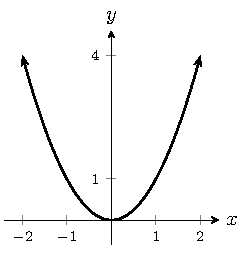
\includegraphics{figuras/x2-total.pdf}\\[2pt]
                $f$
            \end{minipage}
            \hfill
            \begin{minipage}[t]{0.32\textwidth}
                \centering
                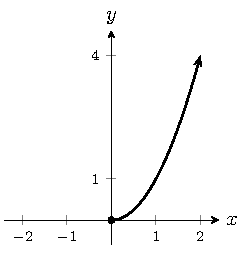
\includegraphics{figuras/x2-0-inf.pdf}\\[2pt]
                $f|_{[0,\infty)}$
            \end{minipage}
            \hfill
            \begin{minipage}[t]{0.32\textwidth}
                \centering
                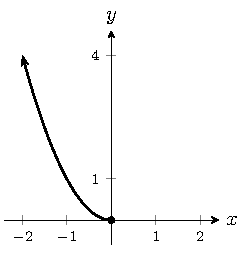
\includegraphics{figuras/x2-inf-0.pdf}\\[2pt]
                $f|_{(-\infty,0]}$
            \end{minipage}

            \vspace{6mm}

            \begin{minipage}[t]{0.32\textwidth}
                \centering
                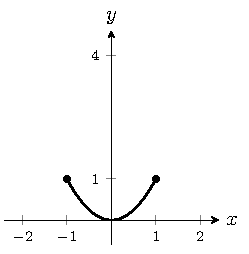
\includegraphics{figuras/x2-cerrado.pdf}\\[2pt]
                $f|_{[-1,1]}$
            \end{minipage}
            \hfill
            \begin{minipage}[t]{0.32\textwidth}
                \centering
                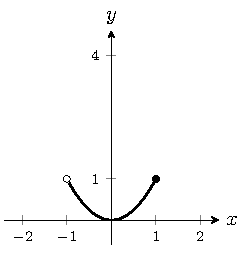
\includegraphics{figuras/x2-abierto-cerrado.pdf}\\[2pt]
                $f|_{(-1,1]}$
            \end{minipage}
            \hfill
            \begin{minipage}[t]{0.32\textwidth}
                \centering
                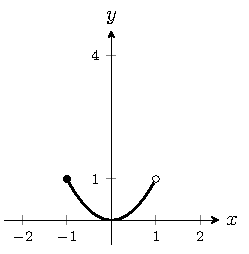
\includegraphics{figuras/x2-cerrado-abierto.pdf}\\[2pt]
                $f|_{[-1,1)}$
            \end{minipage}
        \end{center}
    \end{solucion}

    \begin{problema}
        Determina si las funciones siguientes son pares, impares o ninguna de las dos cosas. Argumenta tu respuesta.
        \begin{multicols}{2}
            \begin{enumerate}
                \item[(a)] $f(x)=\sqrt[3]{x}.$
                \item[(b)] $f(x)=\sin^{2}(x).$
            \end{enumerate}
        \end{multicols}
    \end{problema}

    \begin{solucion}
        \begin{enumerate}
            \item[(a)] $f(x)=\sqrt[3]{x}$.\\
            Sea $x\in\R$. Como
            \begin{equation*}
                \left(-\sqrt[3]{x}\right)^{3}=-x,
            \end{equation*}
            por la unicidad de la raíz cúbica se tiene $\sqrt[3]{-x}=-\sqrt[3]{x}$. Entonces
            \begin{equation*}
                f(-x)=\sqrt[3]{-x}=-\sqrt[3]{x}=-f(x),\qquad\forall x\in\R.
            \end{equation*}
            Por lo tanto $f$ es impar.
            \item[(b)] $f(x)=\sin^{2}(x)$.\\
            Sea $x\in\R$. Como $\sin(-x)=-\sin(x)$, se tiene
            \begin{equation*}
                f(-x)=\sin^{2}(-x)=\left(-\sin(x)\right)^{2}=\sin^{2}(x)=f(x),\qquad\forall x\in\R.
            \end{equation*}
            Por lo tanto $f$ es par.
        \end{enumerate}
    \end{solucion}

\end{document}